\subsubsection{ILC Feasibility}

The International Linear Collider is the most complete of the major collider designs to date and is more technically feasible than the other competitive linear collider design, CLIC. This is in large part due to the lower proposed energy scale and the usage of widely tested, mature technology. Many areas of earlier concern have benefitted from over a decade of R\&D. Key areas requiring further development will be looked at in detail in this section.

The primary technical challenge of the ILC is the large scale production of suitable superconducting radio frequency SCRF main linac (linear accelerator) cavities capable of providing acceleration gradients of 35 MV/m. Also important is the need for further advances in the mitigation of interference between the electron and positron beams and preservation of the vertical emittance. Additionally the requirements of a suitable radio frequency RF power generation system have been considered.

\paragraph{Power Generation}

The RF power requirements are provided by 10MW multi-beam klystrons, converting electron beam energy to radio frequency waves for the driving of the acceleration linacs at efficiencies of up to 80\% \cite{LINAC:Klystron}. These have surpassed the desired specifications and are available from a number of sources worldwide. The MBK's are to be driven by 120 kV Marx modulators, converting out-of-the-wall AC power to the fine-tuned requirements of the accelerator. This design is still in a stage of prototype optimisation at the SLAC National Accelerator Laboratory where it was proposed and developed \cite{LINAC:Marx}. The solid-state design of the Marx offers advantages over the traditional oil-filled transformer design: compactness, performance flexibility and lower cost. However the designs require further extended period tests to prove fully capable.

The multi-beam klystron design to be used as a baseline has previously seen use at the European XFEL Linac. At this facility the MBK modules produced 1.5ms pulses at a rate of 10 Hz at an efficiency of 65\% \cite{LINAC:KlystronsXFEL}. To account for future upgrades to the reach of ILC, the linac will need to be capable of accelerating 9 mA of beam current. Multiple cavities will be driven by each 10 MW power source depending on beam current and configuration parameters. This necessitates designs that permit remotely adjustable power ratios supplied to each group of linacs, driving them at the maximum gradient with the minimum losses.
Two separate ideas for the transportation of power to the linacs have been proposed and one must be settled upon following analysis of the benefits. Firstly a Distributed Klystron Scheme: both klystrons and modulators are positioned along the main tunnel and shielded. Each supplies groups of up to 39 cavities. This is a robust proposition that has seen rigorous testing at the superconducting RF facility at KEK-STF \cite{IPAC:DRFSTest}. Additionally this design predicts lower maintenance and replacement cost overheads due to the accessibility of the modules by siting them along the main tunnel \cite{LINAC:DRFS}.

The alternative to this is a Klystron Cluster Scheme, the klystrons are housed in buildings on the surface above the tunnel. 19 klystrons in each station provide power that is combined into a single 0.5 m diameter waveguide and transported down to the acceleration tunnel to be periodically tapped off over a range of about one kilometre. Proof of principle testing over the period 2011\textendash 13 has provided a good argument for the capabilities of this method at the power levels required by the ILC \cite{IPAC:Klystron}. The KCS is attractive as it reduces the required underground footprint and moves most of the facility's waste heat generation to the surface where it is relatively easily removed. These cost saving factors are balanced against the need for surface installations roughly every 2 km and the need for further R\&D to reduce increased losses in the combined waveguide. Assuming sufficient research into this issue, the choice largely comes down to necessities of the chosen site, a flat topography favours the KCS, whereas a more contoured surface would dictate DKS as the preferred option.

\paragraph{SCRF Cavities}

Cost-effective large scale production of components is at present a major challenge facing the project. The construction of the SCRF linacs is a primary cost-driver, after cost of the tunnel. Approximately 16,000 cavity cells assembled into 1,700 cryomodules are projected to be needed \cite{ILC:PIPReport}, and the demands that this quantity of high-tech component production places on the industry are significant. The required gradient of 35 MV/m has been successfully achieved on a prototype scale at key sites around the globe: Fermilab and Jefferson Lab in North America, KEK in Asia and DESY in Europe. The scale of production necessary for a project the size of ILC remains the primary consideration.

Development of the production capacity has been driven forward by the European X-ray free-electron laser XFEL, a project that represents the current largest scale implementation of the technology. A 17.5 GeV SCRF linac produced by 80 cryomodules comprising a total of 640 cavities. This is a fraction of that required for the ILC but stands as a prototype case and provides a good model for the global coordination necessary to achieve the required rate of supply. Using a model of five vendors providing cavities over a 5 year timeline, prior to a two-year ramp-up period, it is estimated that the needs of the project can be met.

The construction process of SCRF modules demands a clean room environment from start to finish and takes place over three industrial steps: niobium refining and product manufacture, cavity forming and surface treatments, and cryomodule assembly \cite{IPAC:Industrialisation}. Testing is required after each stage and rigorously after the final assembly. As in the XFEL project, a model based around a `hub laboratory' may prove the best course of action. In this scenario an accelerator physics laboratory is identified for each region of the globe wherein production takes place. The hub acts as a conduit between the industry sites and the ILC itself, ensuring the performance of the cryomodules shipped to the ILC achieve the specifications and procuring and qualifying the niobium required. 

The labs already possess the infrastructure for such cold tests and could also act as the site for final cryomodule assembly, under contract with industry. Regionally distributed production and supervision by hub locations in the manner described here can be scaled reasonably well to fit the demands of the project; it also provides internal economic benefits to all regions involved in production. The sharing of work across laboratories implicit in this approach is a key part of the process. The complexity of such an approach is significant, however, the use of multiple markets could lead to cost inflation. Collaboration between the hubs is mandatory if this is to be avoided.

The scheme was demonstrated as viable by the S1-Global programme at KEK-STF \cite{IPAC:S1Module}. Collaboration between FNAL, DESY and KEK produced an 8 cavity acceleration module, the component cavities and auxiliary systems having been constructed separately and delivered to KEK. The scheme allowed for direct comparison between 3 variations on the technology, as well as a demonstration of the viability that separate systems be brought together for integration.

Superconducting cavities see a limit in performance due to two main effects: field emission, electron emission due to the proximity of high electric fields and quench, a phenomenon that arises when a specific voltage applied will cause the material to lose all superconducting capabilities. Improvements to the surface treatment phase of production have successfully countered field emission issues at gradients up to the desired 35 MV/m \cite{ILC:TechnicalDesignReport}. Research conducted at Jefferson Lab identified that surface defects in the materials are the primary causes of cavities encountering the quench limit. Localised surface defects were successfully removed by re-melting the niobium material in the vicinity of the defect \cite{SRF:Gradient}. The ILC baseline design 9\textendash cell cavities were demonstrated to be capable of 90\% gradient yield at 38 MV/m \cite{IPAC:SRFGradient}.  

\paragraph{Beam Interference}

The transferal of the electron and positron beams from the damping rings to the main linacs involve ramping up the energy of the beams from 5\textendash 15 GeV. During this process synchrotron radiation can build up an electron cloud in the evacuated chambers of one beam that leads to instabilities in the other. This process affects the 6 dimensional phase-space of the oppositely charged beam of particles, raising a factor of this phase-space known as the vertical emittance \cite{SSolutions:BeamEmittance}. The emittance carries information about the quality of the beam; beams with larger values of emittance are both difficult to transport in a coherent and maintained manner and experience complications when undergoing transfer from one section of the machine to another \textendash the SCRF linacs to final focusing stage for example.

The long bunch length prior to compression and large energy spread of the beam after compression both compound the issue. Systems to monitor the emittance values and tune the system accordingly are mandatory to achieve the desired design value of emittance of 37nm. Emittance preservation will come from precise manipulation of the magnetic fields to continually correct the trajectory and collimation sections that remove beam-halo particles travelling in the wake of the main beam that would otherwise produce background readings in the detectors at the interaction point. Simulations of the performance of the analytical tools and software required to carry out these tasks give promising results for implementation \cite{PAC:Emittance}. The most successful physical implementations to date have occurred at the ATF2 final-focus experiment at KEK, a prototype damping ring performing under the ILC specifications with beam-line optics aiming at local correction of the bunches. As of December 2012 ATF2 achieved a beam emittance of 70 nm and continues to focus in on the objective value with collaboration from other studies around the globe \cite{ATF2}.

\subsubsection{CLIC Feasibility}

Compared to the ILC, the Compact Linear Collider (CLIC) is facing more technical feasibility challenges as it boasts a much higher energy reach of 3 TeV and a luminosity of $2 \times 10^{34}$ $cm^{-2} s^{-1}$, beyond the reach of standard superconducting technology proposed for the ILC. Hence, new previously-untested technology is being proposed for CLIC in order to achieve the proposed technical goals \cite{CLIC:ArticleSymmetry}. In this section, a critical assessment of the technical feasibility of CLIC is carried out.

The two main technologies currently proposed for CLIC that pose the greatest feasibility challenge are the 100 MV/m linac gradient in the accelerating structure, and the two-beam acceleration scheme used to generate and extract power from the drive beam of electrons and positrons. The challenge of producing an ultra-low emittance beam is also addressed \cite{CLIC:Concept}.

\paragraph{Accelerating Gradient}

The energy E of the colliding beams is given by equation \ref{eq:CollidingBeamsE} \cite{CLIC:Concept}:

\begin{equation}
    E = E_{acc} L F
    \label{eq:CollidingBeamsE}
\end{equation}

where $E_{acc}$ is the average loaded gradient of the accelerating structures, L is the length of each linac and F is the ``fill factor'', which characterises the fraction of the linac occupied by accelerating structures. It is the general case for colliders such as the ILC and CLIC that in order to reduce overall construction cost, reducing L is of key importance here, without compromising the energy reach E of the collider. Minimising the value of L also allows for a compact collider that eases the siting of the accelerator complex. Hence, in order to maximise E, high fill factors and high gradients are required.

The proposed value of 100 MV/m for the accelerating gradient was chosen as the optimal value while finding a suitable compromise between gradient and performance of the collider, characterised by the figure of merit $L_{bx} \cdot \eta /N$, which measures the ratio of beam luminosity to linac input power ($L_{bx}$ is the luminosity per bunch crossing). In general, the performance increases with decreasing gradient, as seen in Fig. \ref{fig:CLIC:Feasi1}, plotted for figure of merit and total cost against accelerating gradient, for different frequencies of RF power.


\begin{figure}[!htb]
    \centering
    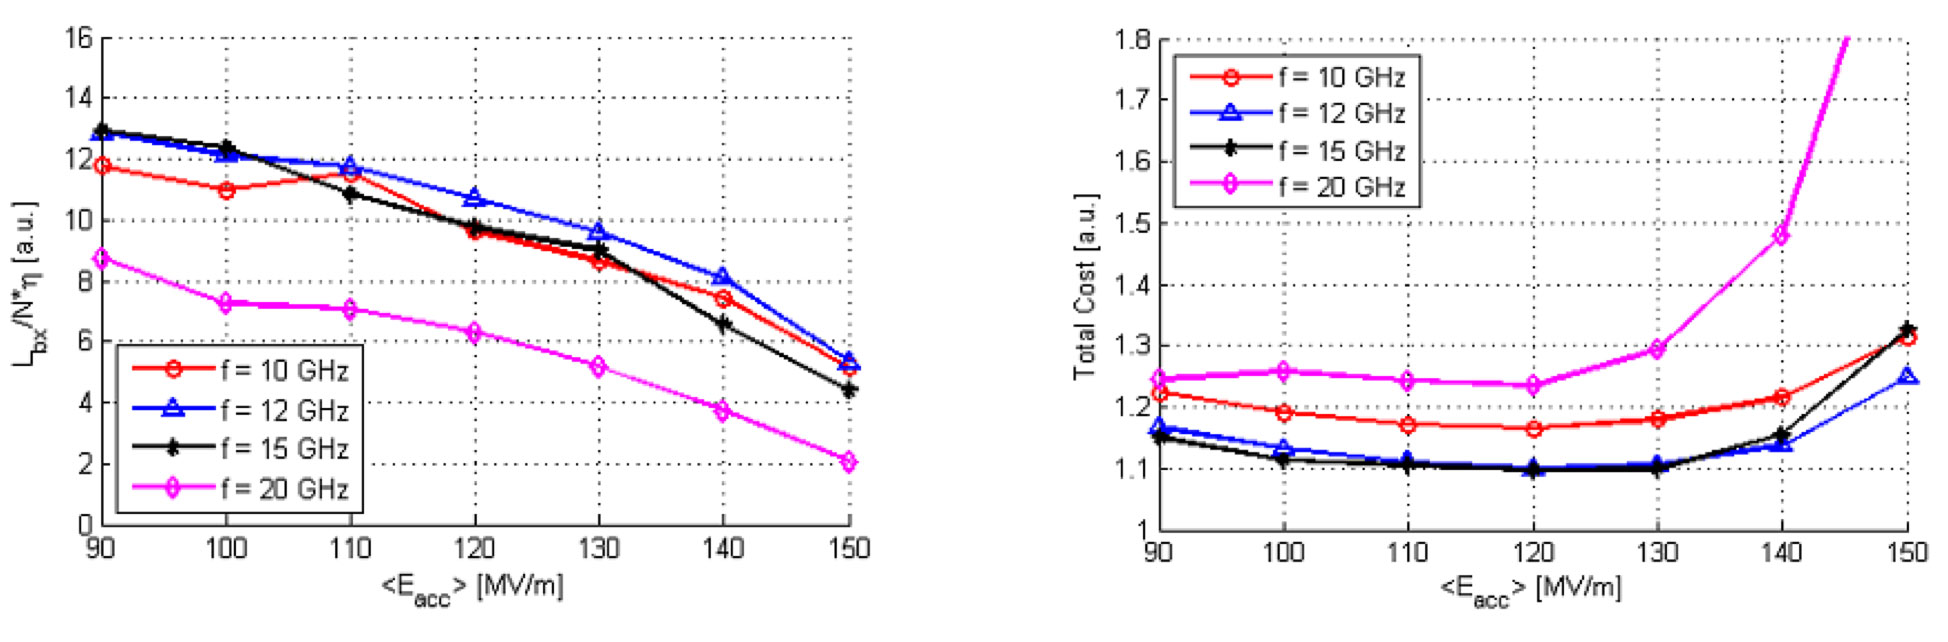
\includegraphics[width=1\textwidth,natwidth=1948,natheight=642]{CLIC_Feasi1.jpg}
    
    \caption{Graph of Figure of Merit and Total Cost against accelerating gradient. These graphs are used to carry out optimisation tests based on cost and luminosity for the optimal value of accelerating gradient. \cite{CLIC:Concept}}
    \label{fig:CLIC:Feasi1}
\end{figure}

As observed from the first graph, the figure of merit decreases as $E_{acc}$ increases, with a marked decrease in performance at f = 20 GHz. In the cost-$E_{acc}$ graph, it is observed that there is a minimum in cost at $E_{acc}$ = 120 MV/m at all frequencies, with f = 12 and 15 GHz having the lowest cost. However, f = 15 GHz has a lower figure of merit than 12 GHz. The final decision made by the CLIC team was an accelerating gradient of 100 MV/m and an RF frequency of 12 GHz, as a compromise between performance and cost.

However, from the first graph, it would seem that choosing a value of $E_{acc}$ = 110 MV/m at f = 12 GHz might be a more optimal choice. While there is a decrease in performance of about 1.5 a.u. from 100 MV/m to 120 MV/m, there is only a difference in performance of about 0.4 a.u. between 100 MV/m and 110 MV/m, for a decrease in cost of about 0.03 a.u.. It is possible that 100 MV/m was chosen over 110 MV/m due to technological feasibility issues and appearances of sparks in the accelerating structure that results in breakdowns. However, the graphs would suggest a more optimal value could be chosen for a better trade-off between performance and total cost.

With 100 MV/m and 12 GHz, and a fill factor of 78.6\%, the length of each 1.5 TeV linac was calculated to be about 21km. However, with a 110 MV/m gradient, the length of each linac could be shortened to about 19km, as calculated from the previous equation.

The feasibility of constructing an unprecedented high accelerating gradient is currently being tested at the CERN CLIC Test Facility 3 (CTF3), whose main aim is to prove the main feasibility issues with the two-beam acceleration technology \cite{Nuclear:CTF3}. Table \ref{tab:CLIC:Feasi1} compares the CLIC nominal parameter with the current (and planned) parameters of the CTF3 facility.

\begin{table}[!htb]
\makebox[\linewidth]{
    \begin{tabularx}{1.3\textwidth}{X | X | X | X | X}
\textbf{Parameter}                     & \textbf{CLIC Nominal}          & \textbf{2011}                                              & \textbf{2012}                                       & \textbf{2013}                     \\ \hline
    $I_{initial} (A)$             & 4.2                   & 7                                                 & -                                          & -                        \\
    $I_{final} (A)$               & 100                   & 28                                                & 30                                         & -                        \\
    $Q_b$                         & 8.4                   & 4 (2.3 nom.)                                      & -                                          & -                        \\
    Norm. Emittance RMS (mm)      & $\leq$ 150            & 150 (factor 4 comb. beam, vertical)               & $\leq$ 150 (factor 8 comb. beam, vertical) & -                        \\
    Bunch Length (mm)             & $\leq$ 1              & $\leq$ 1 (linac), $\leq$ 2 (CLEX)                 & $\leq$ 1 (CLEX)                            & -                        \\
    E (GeV)                       & 2.4                   & 0.12                                              & -                                          & 0.15                     \\
    $T_{pulse}$ initial ($\mu s$) & 140                   & 1.4                                               & -                                          & -                        \\
    $T_{pulse}$ final ($ns$)      & 240                   & 140 (240)                                         & 140 (240)                                  & 140 (240)                \\
    Beam Load Eff. (\%)           & 97                    & 95                                                & -                                          & -                        \\
    Deceleration (\%)             & 90                    & 26                                                & 35                                         & $\geq$ 50                \\
    Phase Stability at 12GHz      & 0.2                   & -                                                 & 0.5                                        & 1                        \\
    Intensity Stability           & $0.75 \times 10^{-3}$ & $0.5 \times 10^{-3}$ (linac), $10^{-3}$ (comb. 4) & $2 \times 10^{-3}$ (comb. 8)               & $\leq 10^{-3}$ (comb. 8) \\
    \end{tabularx}
    }
\caption{Major parameters at the CTF3 facility, as compared to CLIC nominal values. The goal values of the parameters are also included. (CLEX – CLIC Experimental Area) \cite{CLIC:Concept}}
\label{tab:CLIC:Feasi1}
\end{table}

\begin{figure}[!htb]
    \centering
    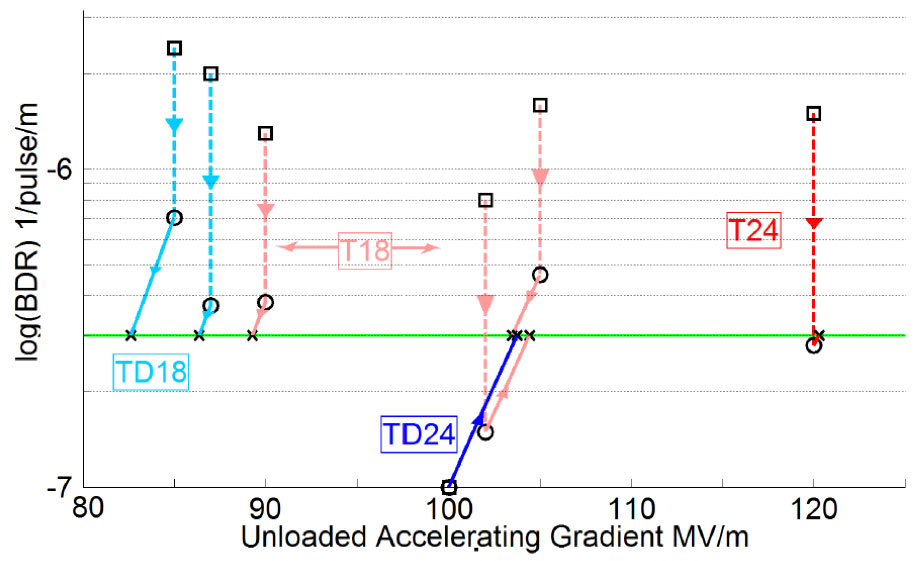
\includegraphics[width=1\textwidth,natwidth=922,natheight=561]{CLIC_Feasi2.jpg}
    
    \caption{Performance of different accelerating structures (T18, TD18, T24 and TD24), scaled to the nominal breakdown rate (BDR). The CLIC allowed BDR is $3 \times 10^{-7} m^{-1}$. \cite{ICFA:BeamDynPress}}
    \label{fig:CLIC:Feasi2}
\end{figure} %

Figure \ref{fig:CLIC:Feasi2} shows the achieved accelerating gradients at different generations of accelerating structures (T18 and TD18 are the early designs). The T24 structure had demonstrated an unloaded accelerating field of more than 120 MV/m, while the TD24 structure, which has been equipped with damping slots (i.e. the CLIC baseline structure), demonstrated an accelerating gradient of 97 MV/m at a breakdown rate of $5 \times 10-5 m-1$. While the gradient is very close to the nominal value of 100 MV/m, the breakdown rate is still about two orders greater than the allowed breakdown rate at CLIC of $3 \times 10^{-7} m^{-1}$.

CTF3 is currently scheduled to run till 2016 \cite{ICFA:BeamDynPress} to perform more detailed tests on the demonstrated drive beam generation and two-beam acceleration. However, a limitation to these tests is the low repetition rate due to limited shielding of the CTF3 facility, resulting in the inability to measure accelerating structures at the nominal breakdown rate. Future programs will have to seek to gain greater access to X-band power stations in order to further improve the behaviour and performance of accelerating structures.

\paragraph{Two Beam Acceleration Scheme}

The 100 MV/m accelerating gradient proposed for CLIC is currently beyond the reach of superconducting technology. In order to achieve the necessary energies and accelerating gradient, a two-beam acceleration scheme where the necessary radio-frequency (RF) power is extracted from a low energy drive beam in order to accelerate the main beam of electrons and positrons is being proposed \cite{AccSciTech:Wilson}. Figure \ref{fig:CLIC:Feasi3} shows the schematic layout for CLIC when operating at 3 TeV.

In this proposed system, the main beam of electrons and positrons are accelerated to the required multi-TeV range of energies by decelerating a second parallel drive beam of electrons with a higher intensity and power density, but with a much lower energy. The RF power from the drive beam is transferred to the main beam structure via Power Extraction and Transfer Structures (PETS) \cite{CLIC:Concept}. The main beam accelerating structures, as mentioned previously, are normal-conducting structures designed to perform at 12 GHz (X-band) in order to achieve the required high acceleration gradients.

This is a unique acceleration scheme that, compared to the ILC, has never been seen or operated before, let alone on an industrial scale such as the one proposed at CLIC. Hence, there are major technical hurdles to overcome with regards to the two-beam acceleration: these include the generation of the drive beam, the extraction and use of RF power from the drive beam, and the deceleration of the drive beam. \cite{CLIC:Concept}

\begin{figure}[!htb]
    \centering
    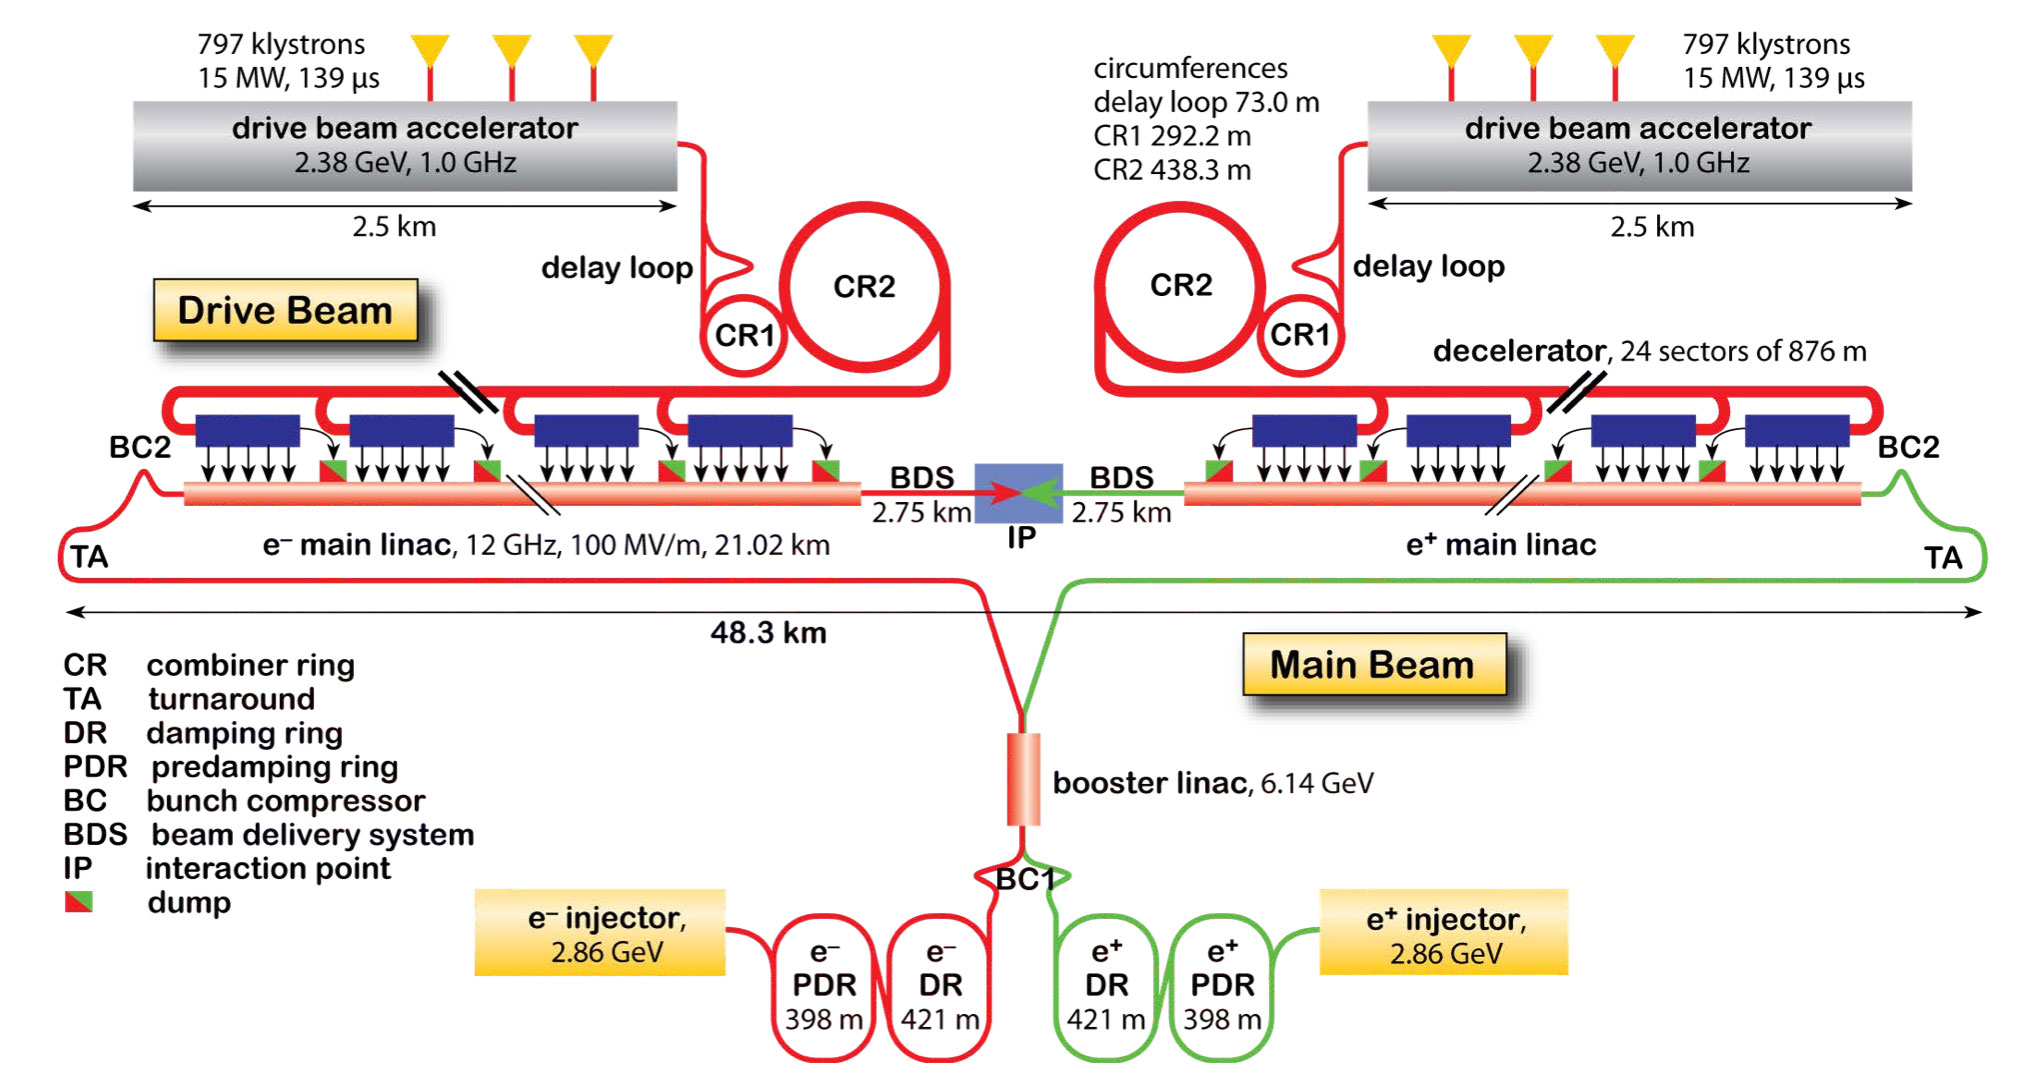
\includegraphics[width=1\textwidth,natwidth=2022,natheight=1092]{CLIC_Feasi3.jpg}
    
    \caption{Schematic layout of the CLIC accelerator complex at 3 TeV. It showcases the novel two-beam acceleration scheme, where the main beam of leptons is powered by a parallel low energy drive beam, whose power is extracted through deceleration in the decelerator. \cite{CLIC:Concept}}
    \label{fig:CLIC:Feasi3}
\end{figure}

\begin{table}[!htb]
\begin{center}
\begin{tabular}{l | c | c | c}
\textbf{Parameter}                & \textbf{Unit}    & \textbf{CLIC} & \textbf{CTF3} \\ \hline
    Accelerated Current      & A       & 4.2  & 3.5  \\
    Combined Current         & A       & 101  & 28   \\
    Accelerated Pulse Length & $\mu$s & 140  & 1.6  \\
    Final Pulse Length       & ns      & 240  & 140  \\
    Acceleration Freq.       & GHz     & 1    & 3    \\
    Final Bunch Freq.        & GHz     & 12   & 12   \\
\end{tabular}
\caption{Major drive beam parameters of CLIC and CTF3. \cite{CLIC:Concept}}
\label{tab:CLIC:Feasi2}
\end{center}
\end{table}

At previous CERN facilities CTF1 and CTF2, proof of principle of the two-beam acceleration scheme had already been demonstrated at low energy and low intensity beams \cite{Nuclear:CTF3}. The energies and intensities at CTF3 are relatively higher; however it must be noted that, compared to the required CLIC values (drive beam intensity of 100 A, drive beam energy of 2.75 – 2.86 GeV), the achieved values at CTF3 for drive beam intensity are about 30 A and energies of only 100 – 200 MeV. A list of the major drive beam parameters has been included in Table \ref{tab:CLIC:Feasi2} for comparison.

In order to better test the feasibility of this proposed two-beam acceleration scheme, the Two-Beam Test Stand (TBTS) \cite{Nuclear:CTF3} was constructed at CTF3, which is an experiment that consists of two parallel electron beam lines, simulating the CLIC two-beam layout. TBTS uses a prototype accelerating structure similar to the one that will be used in CLIC, along with an extra-long PETS to compensate for the decreased beam intensity. This is to ensure TBTS is able to investigate the effects of RF breakdowns in the accelerating structures on the beams at the same RF power level and accelerating gradient as found in CLIC \cite{Nuclear:CTF3}.

As mentioned previously, CTF3 has been able to successfully demonstrate drive beam generation and the two-beam acceleration scheme proof of principle in the CDR period. In fact, a 145 MV/m accelerating gradient has been achieved at CTF3 in a baseline CLIC structure \cite{CLIC:Concept}.

\begin{figure}[!htb]
    \centering
    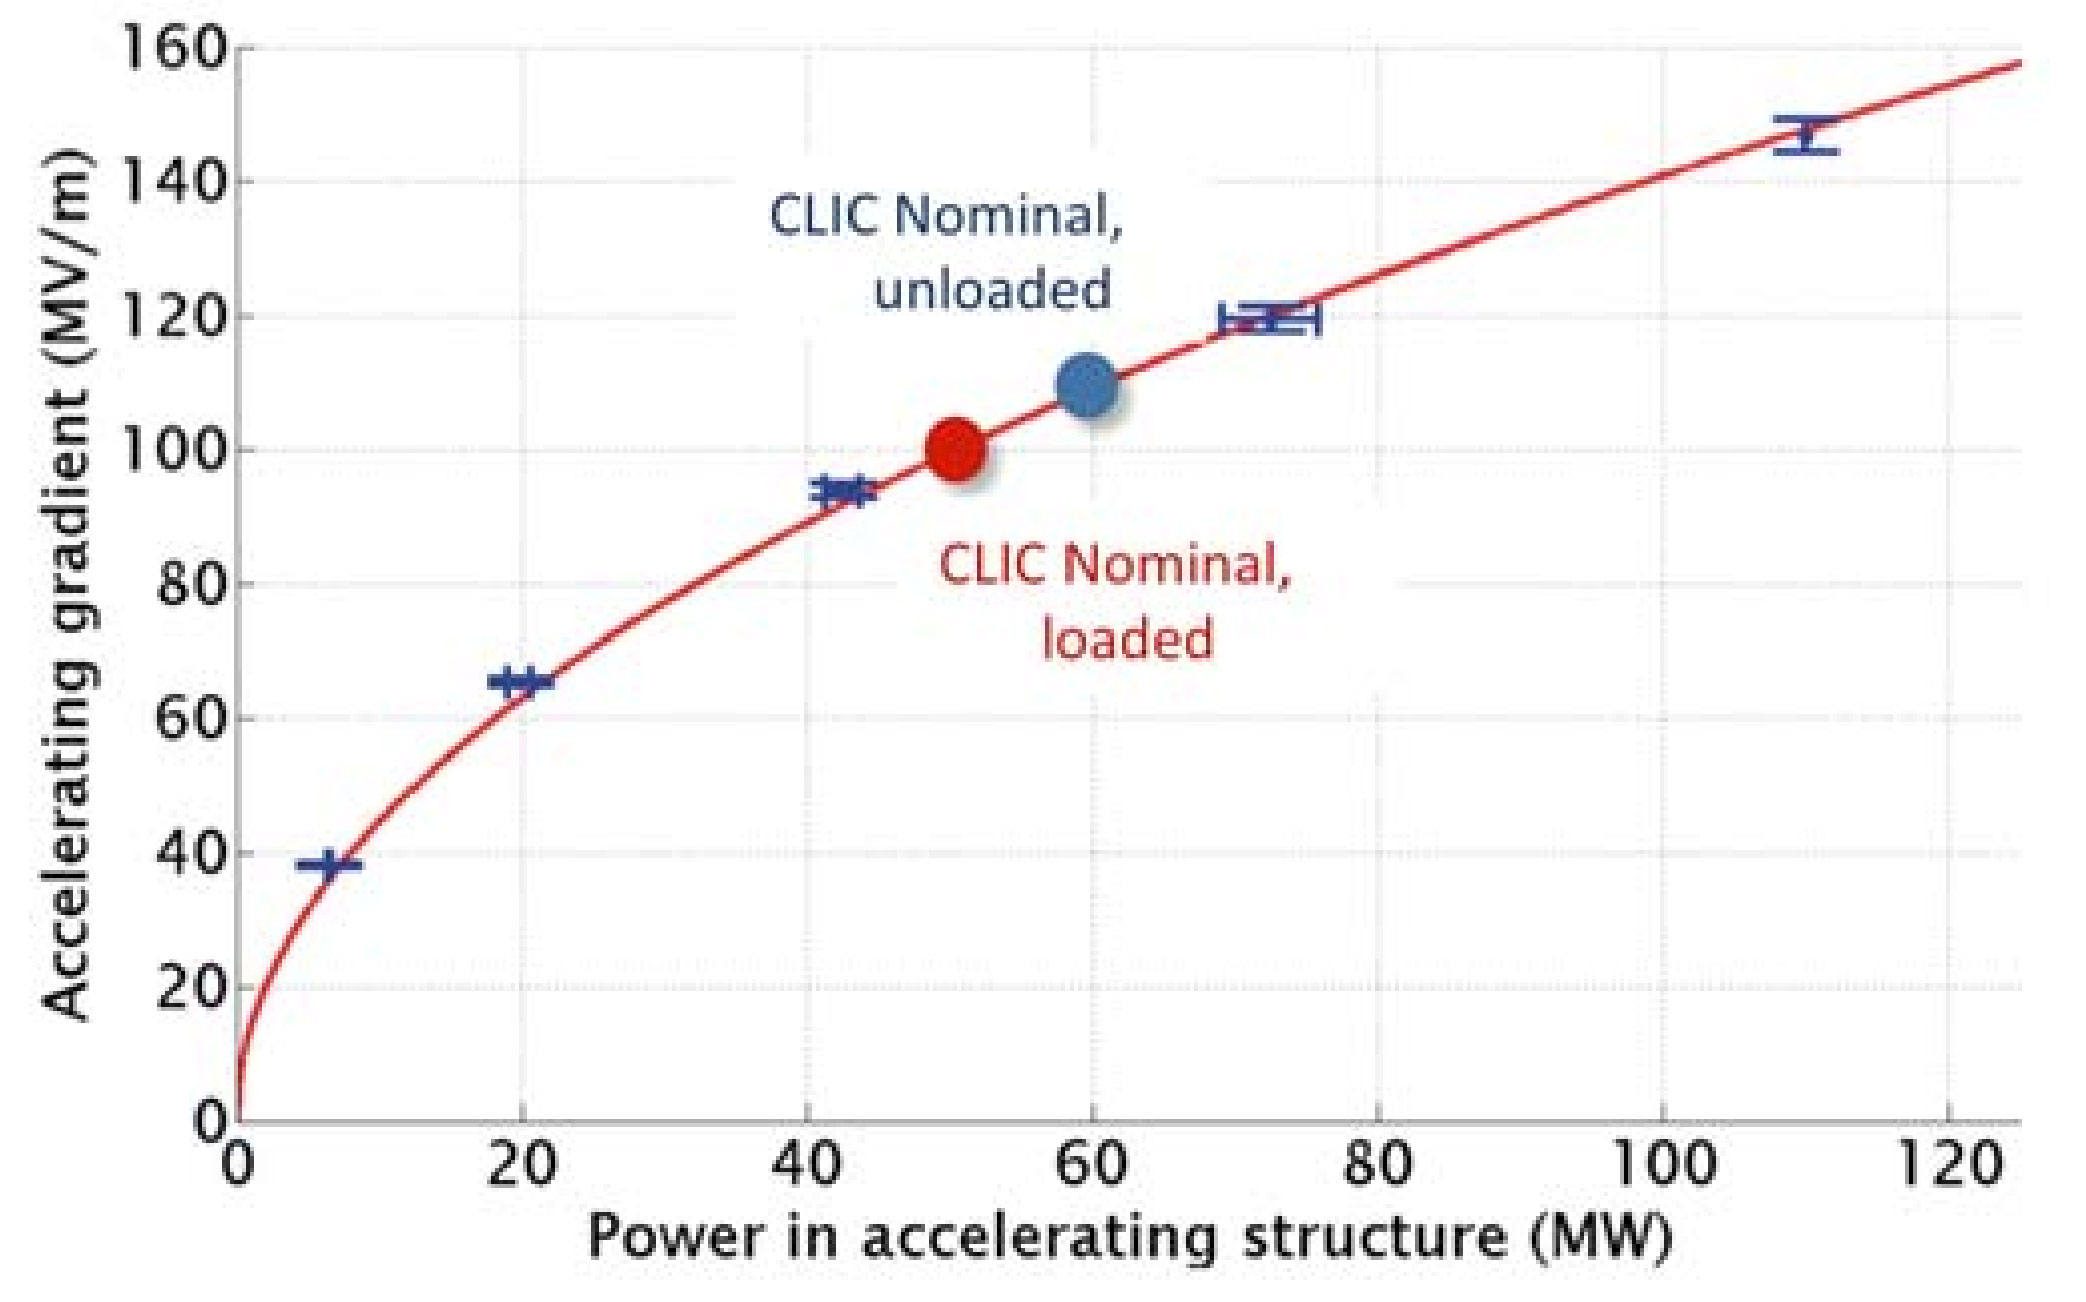
\includegraphics[width=1\textwidth,natwidth=2086,natheight=1302]{CLIC_Feasi4.jpg}
    
    \caption{Graph of experimental results for two-beam acceleration gradient in the baseline CLIC structure (TD24), up to and beyond the nominal CLIC acceleration value. \cite{ICFA:BeamDynPress}}
    \label{fig:CLIC:Feasi4}
\end{figure}

Figure \ref{fig:CLIC:Feasi4} shows the measured gradient in the TD24 accelerating structure, up to and beyond the nominal CLIC values. However, full prototypes of the CLIC modules still remain to be tested to ensure that the previous successful demonstrations can be carried out at the larger CLIC scale. A high efficiency 1 GHz multi-beam klystron and modulator is currently planned to be tested at CERN in 2015-2016 \cite{ICFA:BeamDynPress}, which will provide a more complete system test of a CLIC linac module.

The latest results from CTF3 have also demonstrated drive beam combination by a factor four with the nominal emittance of 150$\mu m$ in both planes. (At CTF3, a 3 GHz, 4 A beam is injected into the combiner ring, where it is stacked up to produce the required 12 GHz beam with a pulse of 280ns, which is referred to as a factor four combination.) The next and final step would be to demonstrate drive beam combination at a stable factor of eight. This is achieved by alternately injecting and bypassing 140ns segments of a 1.5 GHz linac beam pulse, which results in a train of four 140ns sub-pulses, which can be stacked up to get the required 12 GHz beam with a shorter pulse of 140ns. However, progress in achieving this factor eight combination had been hindered by unforeseen technical issues with the traveling wave tubes \cite{CLIC:Concept}.

Future programs at CTF3 will also see an increase in testing of X-band (12 GHz) structures. Under the project title of XBOX, a second test area called XBOX2 is planned to be commissioned at the end of 2014, with XBOX3 to be commissioned by the end of 2015. This will see more than 40 such klystron structures being tested by 2017 \cite{ICFA:BeamDynPress}. The future of the CLIC project will also see a continuation of studies on power and cost optimisation, including the full CLIC module tests outlined above.

In order to extract maximum power from the drive beam to be converted into RF power for the main beam, the drive beam requires deceleration from about 2.4 GeV to 0.24 GeV \cite{CLIC:Concept}. This poses a technical challenge due to the high beam current of 100 A and the large energy spread, hence instability and energy losses have to be minimised. This is being tested and investigated at the Test Beam Line (TBL) at CTF3.

\begin{figure}[!htb]
    \centering
    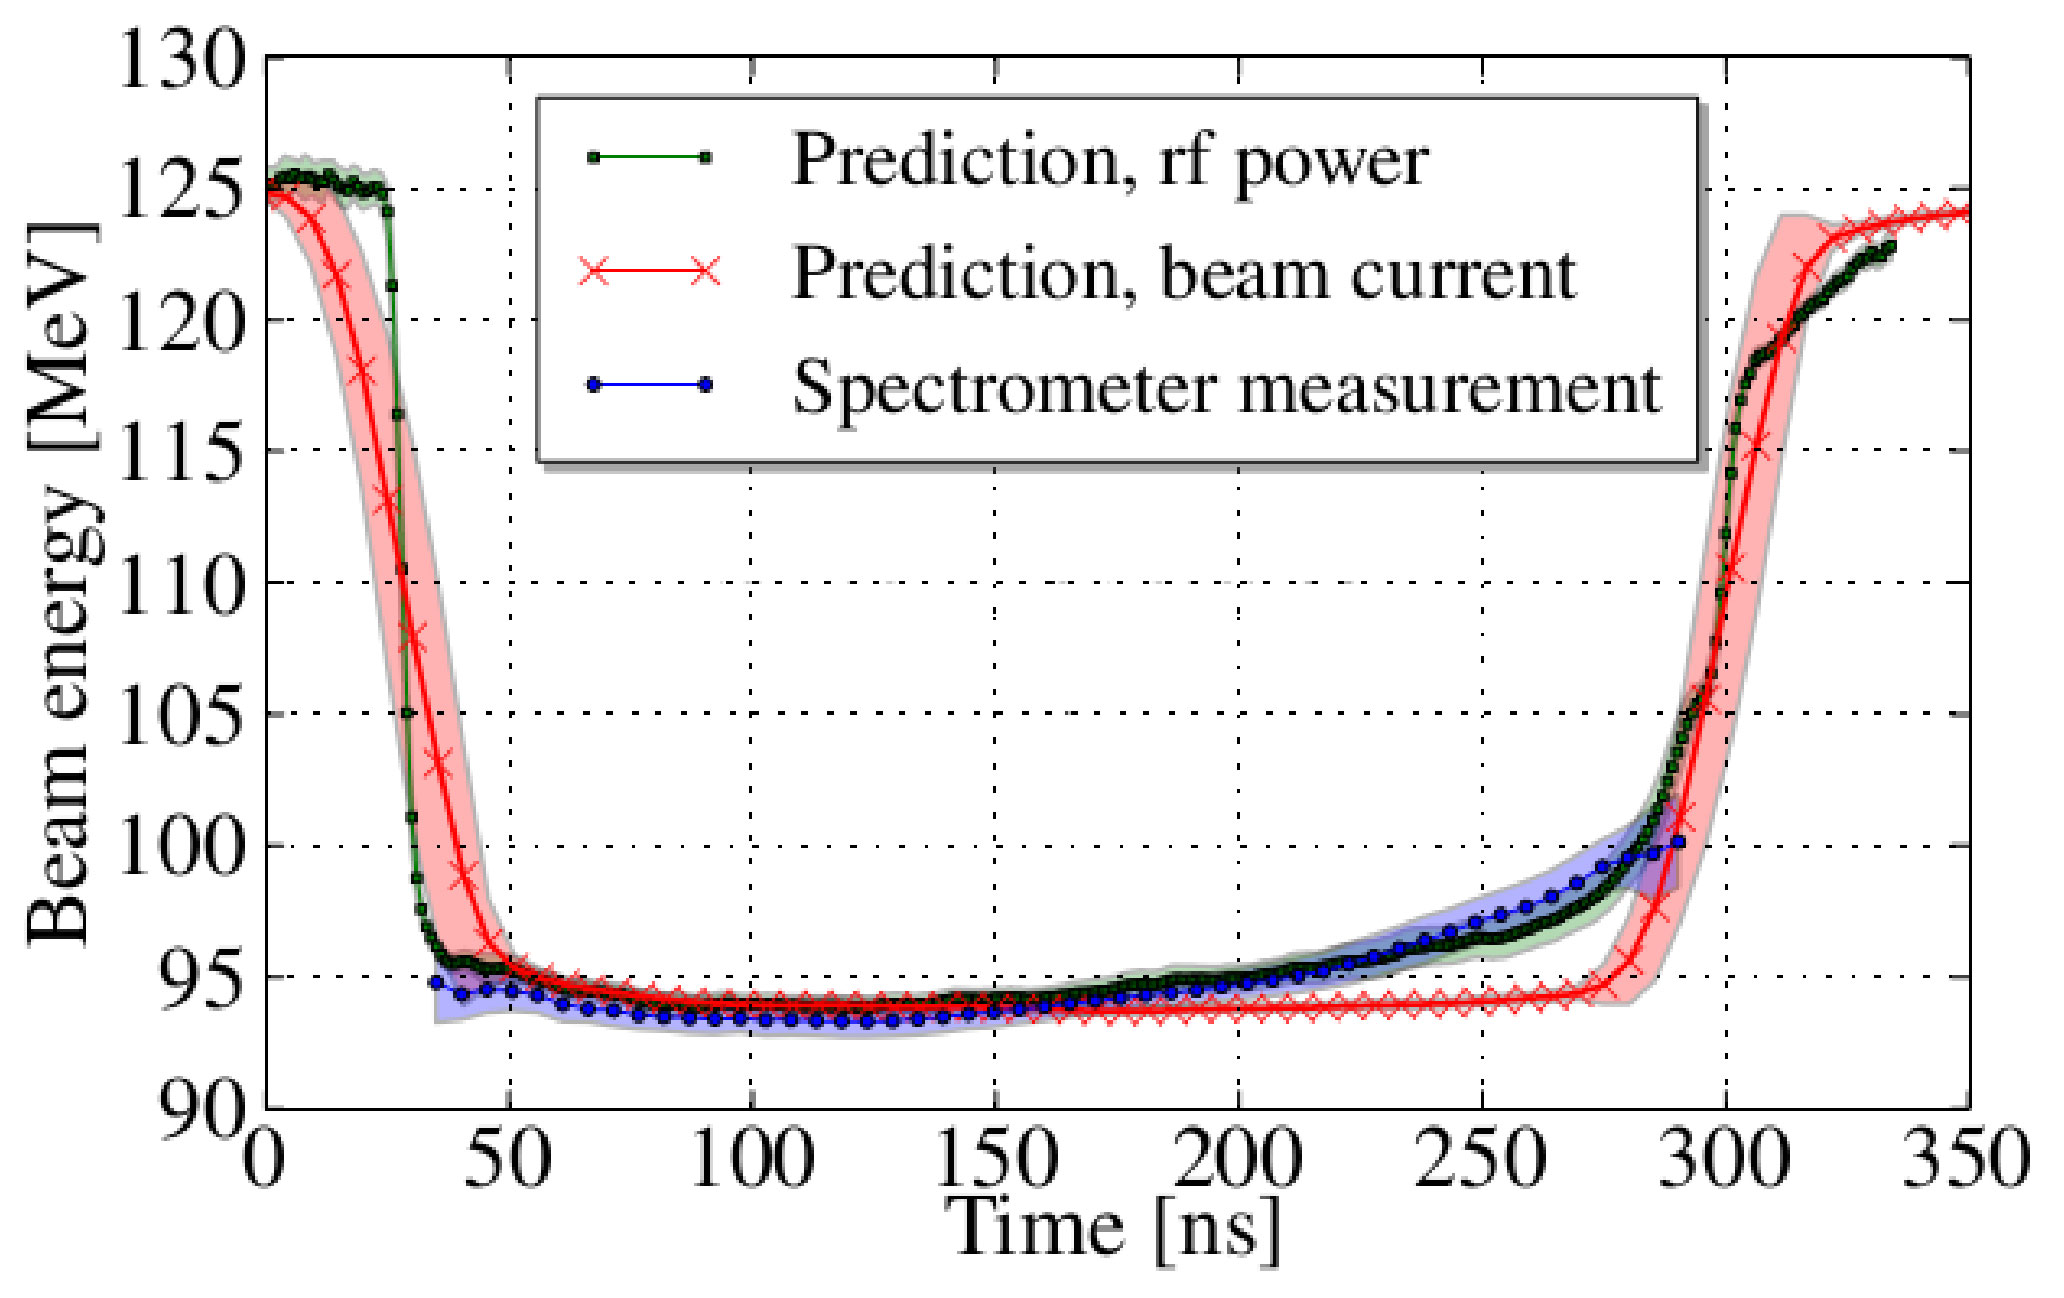
\includegraphics[width=1\textwidth,natwidth=2064,natheight=1298]{CLIC_Feasi5.jpg}
    
    \caption{Graph of beam energy (factor 4 combination) at the end of the Test Beam Line (TBL), with predicted deceleration. (Coloured region represents standard deviations.) \cite{IPAC:TwoBeamAcc}}
    \label{fig:CLIC:Feasi5}
\end{figure}

As of summer 2012, there were 12 PETS in TBL, and latest results demonstrated a successful 25\% deceleration of a combined beam of factor four \cite{IPAC:TwoBeamAcc}, from 125 MeV to about 95 MeV. Predictions show that with all PETS installed, a 50\% deceleration will be achievable.

Lastly, the building block of the 21km linac is the two-beam module (TBM). Currently, there have been five TBM designs with four of them built (two with no quadrupoles, one with a short quadrupole and one with a long quadrupole). Initial string tests have confirmed the feasibility and operation capability of TBMs in preserving the effective accelerating field.

While a second generation of modules is being prepared for future tests, it must be noted that a module length of 2m (due to compact integration of module components) would mean a large number of modules required for the entire length of the linac. Future programs would require major critical assessments of the module and accelerating structure length in order to drive the total cost down \cite{CLIC:Concept}.

\paragraph{Generation of Ultra-Low Emittance Beams}

Besides considering the energy feasibility of CLIC, there is a need to consider the luminosity L of the beam, which is ultimately related to the beam emittance $\epsilon$. Beam emittance is defined as the average spread of particle coordinates in position and momentum phase space. The luminosity of the beam in a linear collider is given by \cite{CLIC:Concept}:

\begin{equation}
    L = H_D \frac{N^2}{\sigma_x \sigma_y} n_b f_r
    \label{eq:BeamLuminosity}
\end{equation}

where $N$ is the number of particles per bunch, $n_b$ is the number of bunches per pulse, $f_r$ is the linac repetition rate, $H_D$ is a correction factor and $\sigma$ is the r.m.s. beam size at collision point, given by:

\begin{equation}
    \sigma = \sqrt{\frac{\epsilon \beta}{\gamma}}
\end{equation}


where $\beta$ is the beta function at collision point, and $\gamma$ is the beam energy normalised to the electron rest energy (0.511 MeV). (The beta function is a Twiss parameter in beam optics, related to the transverse size of the beam as well.)

However, another factor that is of importance, which was previously mentioned, is the figure of merit $M$ (which is defined as the luminosity per wall-plug power $P_{AC}$ for a given beam energy and number of photons emitted in the collision). This is given by (at the high energy regime of 3 TeV):

\begin{equation}
    M = \frac{L}{P_{ac}} \propto \eta \frac{1}{\sqrt{\sigma_z}\sqrt{\epsilon_y}}
\end{equation}


where $P_{AC}$ is the wall-plug power and $\eta$ is the wall-plug-to-beam conversion efficiency.

Hence, we can see that the luminosity (and ultimately the performance of the collider) is dependent on the beam emittance, which has to be minimised in order to increase beam luminosity for high performance. A beam with minimal emittance would mean the particles are confined to a smaller region in space and possess the same momentum – this would increase the probability of particle interactions at collision and hence increase luminosity.

In order to achieve these low emittances, the main beam will be made to radiate synchrotron radiation when circulating through damping rings before entering the main beam linac \cite{CLIC:Concept}. However, the main challenges are the required emittance parameters (500nm and 5nm horizontal and vertical normalised emittance), which are unprecedentedly small.

\begin{table}[!htb]
\makebox[\linewidth]{
\begin{tabularx}{\textwidth}{X | c | c | c}
    \textbf{Parameter}                   & \textbf{Injected} & \textbf{Injected}      & \textbf{Extracted} \\ 
    & $e^-$ & $e^+$ & $e^+ e^-$ \\
    \hline
    Bunch Population ($10^9$)            & 4.3      & 6.6             & 4.1                   \\
    Normalised Horizontal Emittance & $10^5$ mm   & $7 \times 10^6$ mm & 500 mm                   \\
    Normalised Vertical Emittance & $10^5$ mm   & $7 \times 10^6$ mm & 5 mm                     \\
\end{tabularx}
}
\caption{Required parameters of the beam before injection and at extraction from the damping rings (emittance parameters). \cite{CLIC:Concept}}
\label{tab:CLIC:Feasi3}
\end{table}

The feasibility of producing such low emittance beams is currently being investigated at the Accelerator Test Facility (ATF) \cite{KEK:ATF} in the High energy Accelerator Research Organisation (KEK) \cite{KEK}. The results from ATF are listed in the Table \ref{tab:CLIC:Feasi4}.

Currently, ATF has only achieved emittances of 3800nm and 15nm in the horizontal and vertical directions, which are a factor of 7.6 and 3 higher than the required CLIC emittances at 3 TeV. Hence, emittance generation (and there CLIC beam luminosity) still poses as a major challenge – future programs aim to develop new light sources (NSLSII or MAXIV) which would hopefully make new progress in achieving CLIC-like emittances within the next few years \cite{CLIC:Concept}.

\begin{table}[!htb]
\makebox[\linewidth]{
\begin{tabularx}{\textwidth}{X | c | c | c}
    \textbf{Parameter}                   & \textbf{ATF}  & \textbf{CLIC} & \textbf{CLIC} \\
    & & 500GeV & 3 TeV \\
    \hline
    Energy (GeV)                         & 1.3  & 2.86         & 2.86       \\
    Normalised Horizontal Emittance (nm) & 3800 & 1800         & 500        \\
    Normalised Vertical Emittance (nm)   & 15   & 5            & 5          \\
    Particles per Bunch ($10^9$)         & 4    & 7.5          & 4.1        \\
    Number of Bunches                    & 1    & 312          & 312        \\
    Average Beam Intensity (mA)          & 3.5  & 265          & 145        \\
\end{tabularx}
}
\caption{Major parameters related to achieving ultra-low emittances of main beam in the Acceleration Test Facility, compared to the nominal parameter values for CLIC at two energy stages (500 GeV and 3 TeV). \cite{CLIC:Concept}}
\label{tab:CLIC:Feasi4}
\end{table}

\paragraph{Summary}

As outlined in the above sections, the CLIC project is still facing some critical feasibility challenges due to its novel acceleration scheme and required low beam emittance. Many of the parameters have been demonstrated and shown to be feasible. Hence, CLIC remains an attractive alternative for a next-generation multi-TeV lepton collider, capable of reaching energies beyond what the ILC could. However, as the current tests often have different beam parameters than the nominal CLIC parameter values, more research and development is required to ensure that the results achieved currently are directly applicable to a large facility such as CLIC.

Currently, it is safe to estimate that the CLIC project is still in its project preparation phase, and a robust proposal would not only require the completion of the ongoing feasibility tests, but also a consideration of factors such as project cost and power consumption. Hence, more optimisation tests have to be carried out before a mature and realistic proposal can be put forward as a competitor to the ILC. \cite{CLIC:Concept}

\subsubsection{Conclusion}
Considering the magnitude and the variety of technical hurdles that CLIC has to overcome at this 
point, it is clear that the ILC is the better option when it comes to feasibility. While 
the ILC is not free from technical challenges, its main hurdles lie in demonstrating that the required 
technology is viable at an industrial scale. CLIC, on the other hand, requires a previously untested 
acceleration scheme, which includes many technical challenges that are still in the design stage at 
this point. Given the need to maintain the momentum within the particle physics community, it 
would seem sensible to choose the ILC as the more feasible option. 